\documentclass{llncs}
%
%\usepackage{makeidx}  % allows for indexgeneration
\usepackage{graphicx}
\graphicspath{ {./figures/} }
%
\begin{document}

\title{Automatic Estimation of the Optic Nerve Sheat Diameter from Ultrasound Images}
%
\titlerunning{Automatic Optic Nerve Sheat Diameter Estimation} 
% abbreviated title (for running head) also used for the TOC unless \toctitle is used
%
\author{
Samuel Gerber,
Maeliss Jallais,
Stephen Aylward
}

%
\authorrunning{S. Gerber, M. Jallais and S. Aylward} % abbreviated author list (for running head)
%
%%%% list of authors for the TOC (use if author list has to be modified)
%\tocauthor{}
%
\institute{Kitware Inc, Carrboro NC 27510, USA,\\
\email{samuel.gerber@kitware.com}
}

\maketitle              % typeset the title of the contribution

\begin{abstract}
We present an algorithm to automatically estimate the diameter of the optic
nerve sheath from ocular ultrasound images. The optic nerve sheath diameter
provides a proxy for measuring intracranial pressure,  a life threating
condition frequently associated to head trauma. Early treatment of elevated
intracranial pressures greatly improves outcomes and drastically reduces the 
mortality rate. We demonstrate that the proposed algorithm combined with a
portable ultrasound device presents a viable path for early detection of
elevated intracranial pressure in remote locations and without access to trained
medical imaging experts. 
\end{abstract}
%
\section{Introduction}
Portable ultrasound technology is well suited for the development of automated
diagnostics systems that enable emergency responders to quickly assess the
severity of a patient's injuries at accidents. Such light-weight portable
automated systems can be employed in remote environments in which expert medical
imaging personnel and advanced imaging equipment are not readily available.
 
This paper considers the application of a point-of-care, computer-assisted
ultrasound system for in-field traumatic brain injury (TBI) assessment via the
detection of increased intracranial pressure. Delayed treatment of increased
intracranial pressure can cause temporary or permanent brain damage or even
long-term coma and death. For example, it has been shown that acute subdural
hematomas in severe TBI patients cause significant increase in intracranial
pressure, are associated with 90\,\% mortality if detected and treated more than
4 hours after injury, and yet are associated with only 30\,\% mortality if
detected and treated earlier~\cite{Se1981}.

In a clinical setting, a non-invasive approach to measure intracranial pressure is
by ocular ultrasound. From the ocular ultrasound image the physicians manually
measures the diameter of optic nerve sheath at a location 3\,mm behind the retina.
Acquiring such images and making these measurements is challenging and time
consuming task. We propose to automate the process of measuring the diameter of
the optic nerve sheath and integrate within a portable ultrasound system to
automatically report elevated intracranial pressure without the need of manually
measuring the optic nerve sheath diameter. The ultimate goal is a system that is
easy to use and does not require expert personnel or specific training to
diagnose TBI.    

Using ultrasound for estimation of optic nerve sheath diameter is a well
establish approach to diagnose elevated intracranial
pressure~\cite{Ki2008,Ro2011} and various studies have been performed to
establish the optimal threshold for clinical
diagnosis~\cite{Mo2009,Du2011,Ra2011}. But to the best of our knowledge
this is the first time an algorithm is proposed to automate the estimation
process.

\section{Algorithm}
We propose a two step approach to automate the measurement of the optic nerve
sheath diameter. At a high level, the algorithm proceeds by locating the eye
through registration of an ellipse with the largest dark circle in the image
data. From the ellipse an approximate location of the optic nerve is constructed
and used to fit two bars to the walls of the acoustic shadow behind the optic
nerve. This high-level description leaves out several intermediate steps such as
those involving image smoothing, morphological operations, and distance
transforms, described in detail in Section~\ref{sec:details}. that are required
to achieve good registration results.  Figure~\ref{fig:fitted} shows result of
the fitting procedure and illustrates that the proposed algorithm is applicable
to a wide variety of images with differing quality.
\begin{figure}
\centering
\begin{tabular}{ccc}
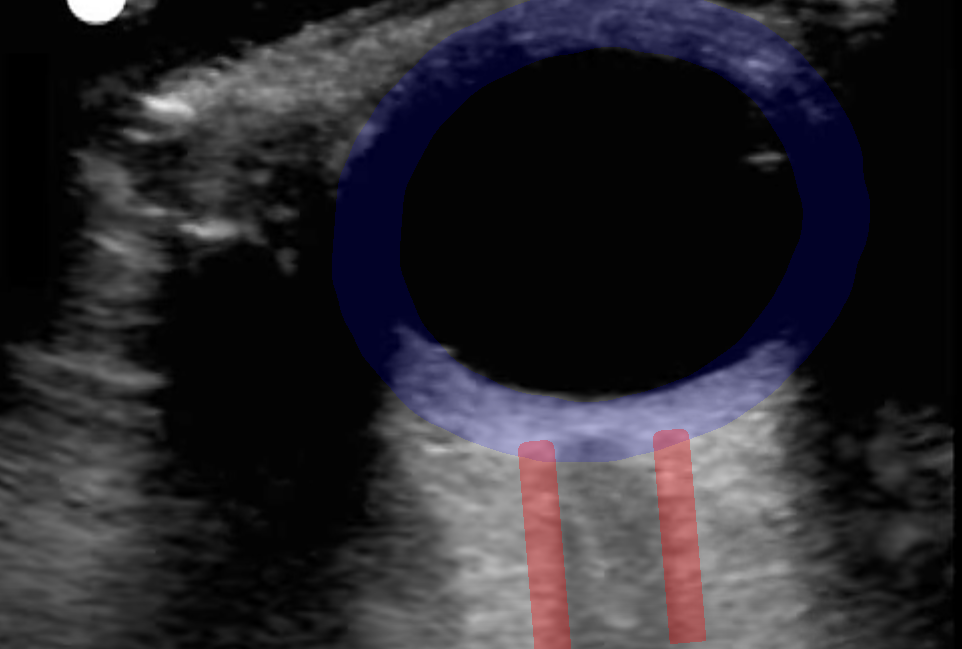
\includegraphics[height=1.2in]{003-overlay.png} &
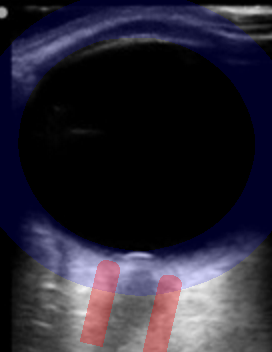
\includegraphics[height=1.2in]{009-overlay.png} &
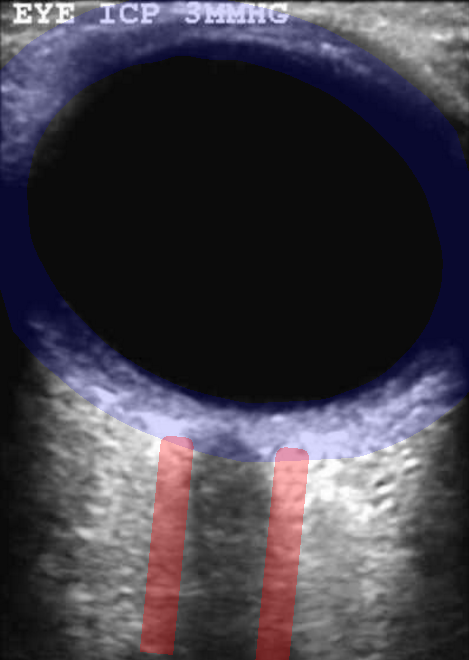
\includegraphics[height=1.2in]{023-overlay.png} 
\end{tabular}
\caption{
\label{fig:fitted}
Result of the proposed algorithm on three ocular ultrasound images. The
overlays illustrate the registration results of the algorithm. The blue ellipse
delineates the location of they eye and the red bars are the result of fitting
the boundary of the acoustic shadow induced by the optic nerve sheath.
}
\end{figure}

\subsection{Algorithm Details}
\label{sec:details}
Here we briefly describe the individual image processing steps to achieve an
algorithm that performs a large variety of images from different types of probes
and differences between subjects.

The first part of the algorithm is locating and estimating the size of the eye.
The liquid of the vitreous body of the eye has very low acoustic impedance and
appears black in B-mode ultrasound images. The boundary of the vitreous body is
frequently clearly delineated through the skin of the closed eye and the
adjacent tissue. However, acoustic shadows, poor probe contact and collagen
floaters cause imperfections in the boundary as well as the interior. Thus, the
proposed eye detection algorithm requires several image processing steps: 
\begin{enumerate}
\item Estimate initial eye center and size:
  \begin{enumerate}
  \item Gaussian smoothing, binary thresholding, morphological closing and
        distance transform.
  \item The maximum distance and its location of the distance transform provide
        initial radius and initial center of the eye orb. 
  \end{enumerate}
\item Refine initial estimates:
  \begin{enumerate}
  \item Distance transform over vertical image strip of width 20 pixels
        around the initial eye center location estimate provides an initial
        minor ellipse radius.
  \item Distance transform over horizontal image strip of width 20 pixels 
        around the initial eye center location estimate provides an initial major
        ellipse radius.
  \end{enumerate}
\item Gaussian smoothing and binary thresholding.
\item Create a binary ellipse annulus with the initial estimates of the minor and
      minor axis of width $0.2$ times the major axis with center located at the
      initial eye center estimate.
\item Register ocular ultrasound (moving image) to ellipse image (fixed image)
      under an affine transform with a masked mean squared error metric. The
      mask is an ellipse that encompasses the ellipse annulus on the fixed
      image. The affine transform is centered on the ellipse center.
\item Refine eye center and major and minor estimates by applying the transform to
      the minor and major axis vectors and the center point.
\end{enumerate}
Figure~\ref{fig:algorithm-eye} illustrates the algorithm for locating the
vitreous body of the eye with several intermediate images of the individual
steps. 
\begin{figure}
\centering
\begin{tabular}{ccccc}
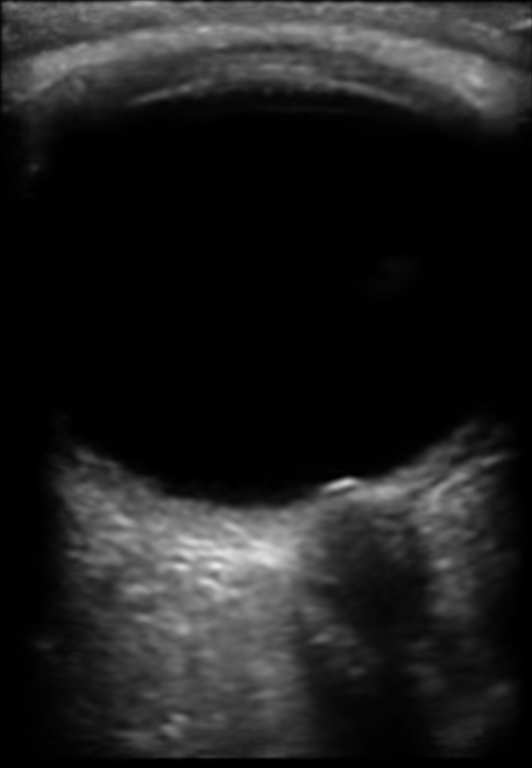
\includegraphics[height=1.22in]{019.png} &

\includegraphics[height=1.22in]{019-eye-smooth.png} &

\includegraphics[height=1.22in]{019-eye-distance.png} &         

\includegraphics[height=1.22in]{019-eye-moving.png} &
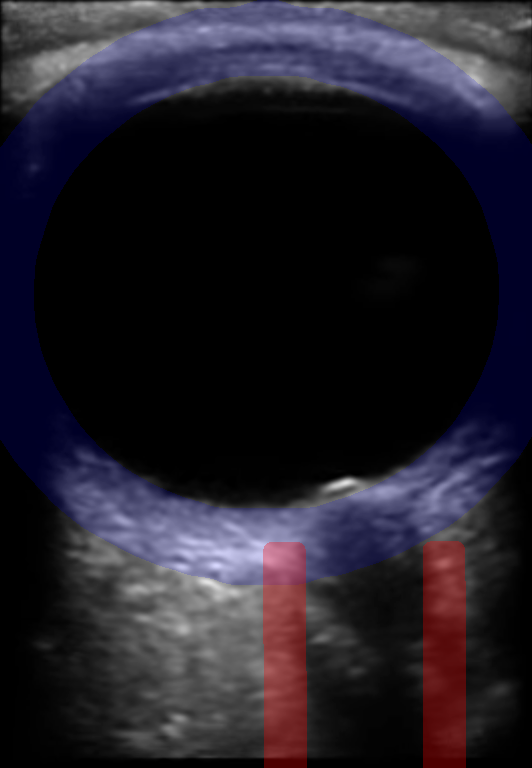
\includegraphics[height=1.22in]{019-overlay.png}\\
(a) & (b) & (c) & (d) & (e)
\end{tabular}
\caption{
\label{fig:algorithm-eye}
Intermediate steps to locate and estimate the size of the eye. (a) Input image,
(b) Gaussian smoothing and threshold, (c) distance transform, (d) the ellipse
image generated from the initial eye location and size estimates and (e) the
registered ellipse and optic nerve sheath (from the nerve estimation algorithm)
overlay on the input image.
}
\end{figure}

The location of they eye provides an approximate region for locating the optic
nerve sheath. The optic nerve sheath has a very strong acoustic impedance and
reflects a significant amount of the energy of the sound wave. This results in an
acoustic shadow that appears as a darker tube behind the optic nerve sheath.
We take advantage of this acoustic shadow to estimate the width the optic nerve.
The shadow again is imperfect and the shadow boundary can exhibit several
imperfections and have strong intensity variations. We suggest the following
image processing steps to enhance the shadow boundary before a registration of
two parallel vertical bars to delineate the width of the shadow:
\begin{enumerate}
\item Extract optic nerve region below the eye using the eye location and size estimates
\item Gaussian smoothing.
\item Scaling of intensities per individual rows alleviate attenuation effects.
\item Compute initial center and width estimates:
  \begin{enumerate}
  \item Binary threshold morphological opening and distance transform.
  \item The maximal distance and its location provide and initial estimate of the
          optic nerve shadow diameter and its location
  \end{enumerate}
\item Scale intensities per row and on each side of the initial optic nerve
      center estimate (Often the left and right boundary exhibit vastly
      different intensities). 
\item Refine initial center and width estimates:
  \begin{enumerate}
  \item Binary threshold, morphological opening and distance transform.
  \end{enumerate}
\item Use refined initial center and width to create an image with two vertical bars. 
\item Register the two vertical bars (fixed image) to the processed image (moving
      image) under a similarity transform (rotation, translation and scaling)
      with a masked mean squared error metric. The mask is a rectangle that
      encompasses the two vertical bars. The similarity transform is centered on
      the initial  center estimate.
\item Refine width estimates by applying the registration transform to a vector
      that spans from the left to the right vertical bar of the fixed image.
\end{enumerate}
\begin{figure}
\centering
\begin{tabular}{cccccc}
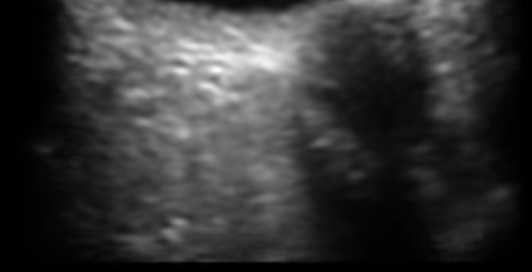
\includegraphics[height=0.36in]{019-nerve.png} &
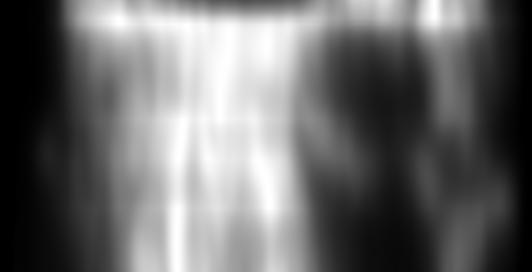
\includegraphics[height=0.37in]{019-nerve-smooth.png} &
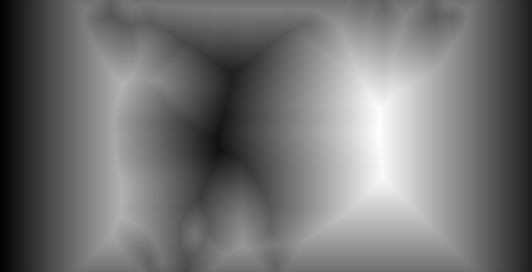
\includegraphics[height=0.36in]{019-nerve-distance.png} &
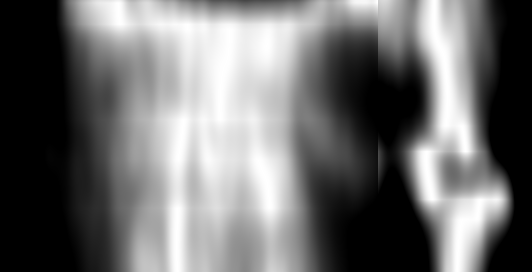
\includegraphics[height=0.36in]{019-nerve-scaled.png} &

\includegraphics[height=0.36in]{019-nerve-thres.png} &         

\includegraphics[height=0.36in]{019-nerve-moving.png} \\         
(a) & (b) & (c) & (d) & (e) & (f)
\end{tabular}
\caption{
\label{fig:algorithm-nerve}
Intermediate steps to fit the acoustic shadow of the optic nerve sheath. (a)
Optic nerve sheath region located from the eye location and size estimates, (b)
Gaussian smooth and intensity scaling of individual rows, (c) Distance
transform, (d) scaling of rows independently left and right of the initial
center (e) thresholding and (f) vertical bars before registration based on intial
estimates.
}
\end{figure}

\subsection{Interactive Graphical User Interface}
\label{sec:gui}
Our algorithm reports estimates of the optic nerve sheath diameter in near real
time as an ultrasound probe is swept across the closed eye of a patient.  This
algorithm is now integrated into a user-friendly interface and performs
estimates at 4 frames per second. Depending on the ultrasound probe, the
algorithm can be simplified by skipping the eye estimation step to run at around
20 frames per second. 
\begin{figure}
\centering
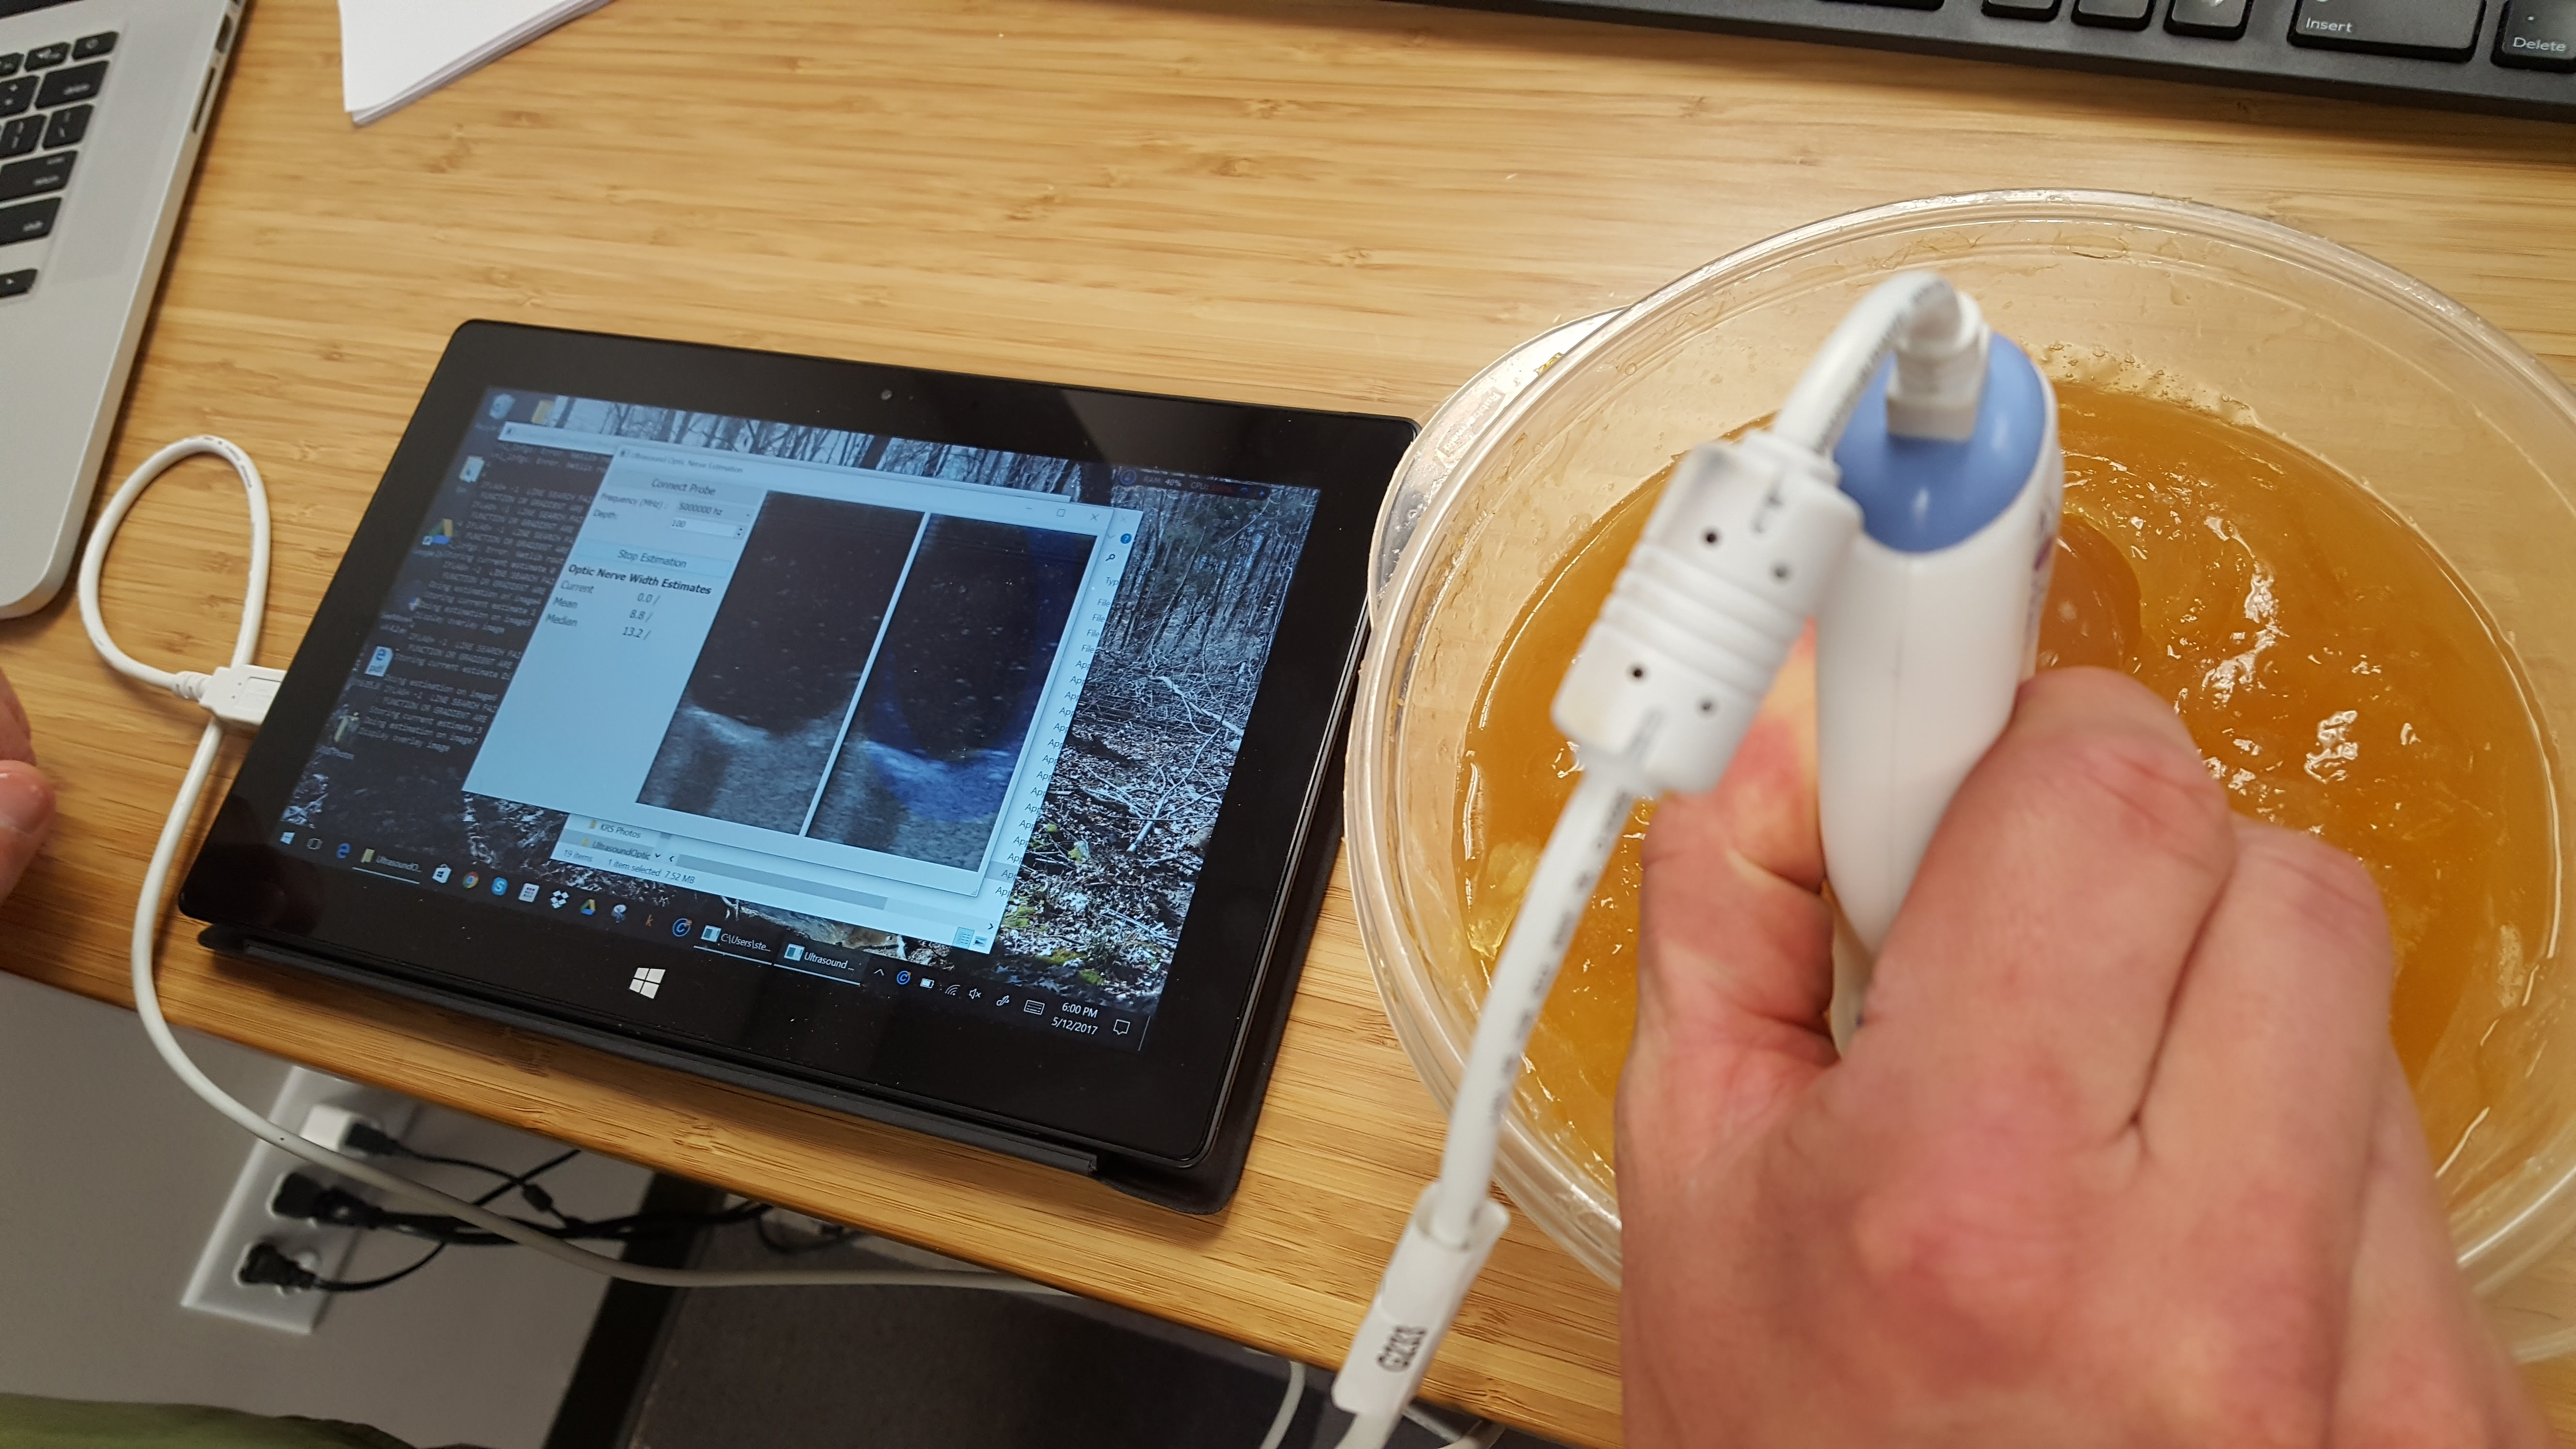
\includegraphics[width=0.7\linewidth]{gui.jpg} 
\caption{
\label{fig:gui}
Graphical user interface to image an eye phantom on a windows table connected to
a USB ultrasound probe from Interson at interactive frame rates. 
}
\end{figure}


\section{Evaluation}
We evaluated the performance of the proposed automatic estimator in two ways.
In Section~\ref{sec:manual} a comparison to manual estimates from novices and
medical experts shows that the method has high precision and performs within the
range of expert variability. Section~\ref{sec:groundtruth} evaluates the
automatic estimates using a gelatine eye phantom with known ground truth
diameters and shows that the method is very accurate. 

\subsection{Comparison to Manual Estimation}
\label{sec:manual}
For this study 13 volunteers ranging novices to medical professionals annotated
23 ocular ultrasound images (in pixel units due to unknown image spacing units).
A linear regression of the automatic estimates with two different parameter
settings against the estimates of a medical expert resulted in an $\mathrm{R}^2$
of 0.82 and 0.91, respectively and both were  statistically significant with a
p-value on the order of machine precision ($2e^{-16}$).

%Figure~\ref{fig:regression} shows a linear regression of the automatic estimated
%diameter from two different parameter settings of the algorithm as compared to a
%medical expert. The automatic estimates had an $\textrm{R}^2$ around 0.91 and
%0.82, respectively. 
%\begin{figure}
%\centering
%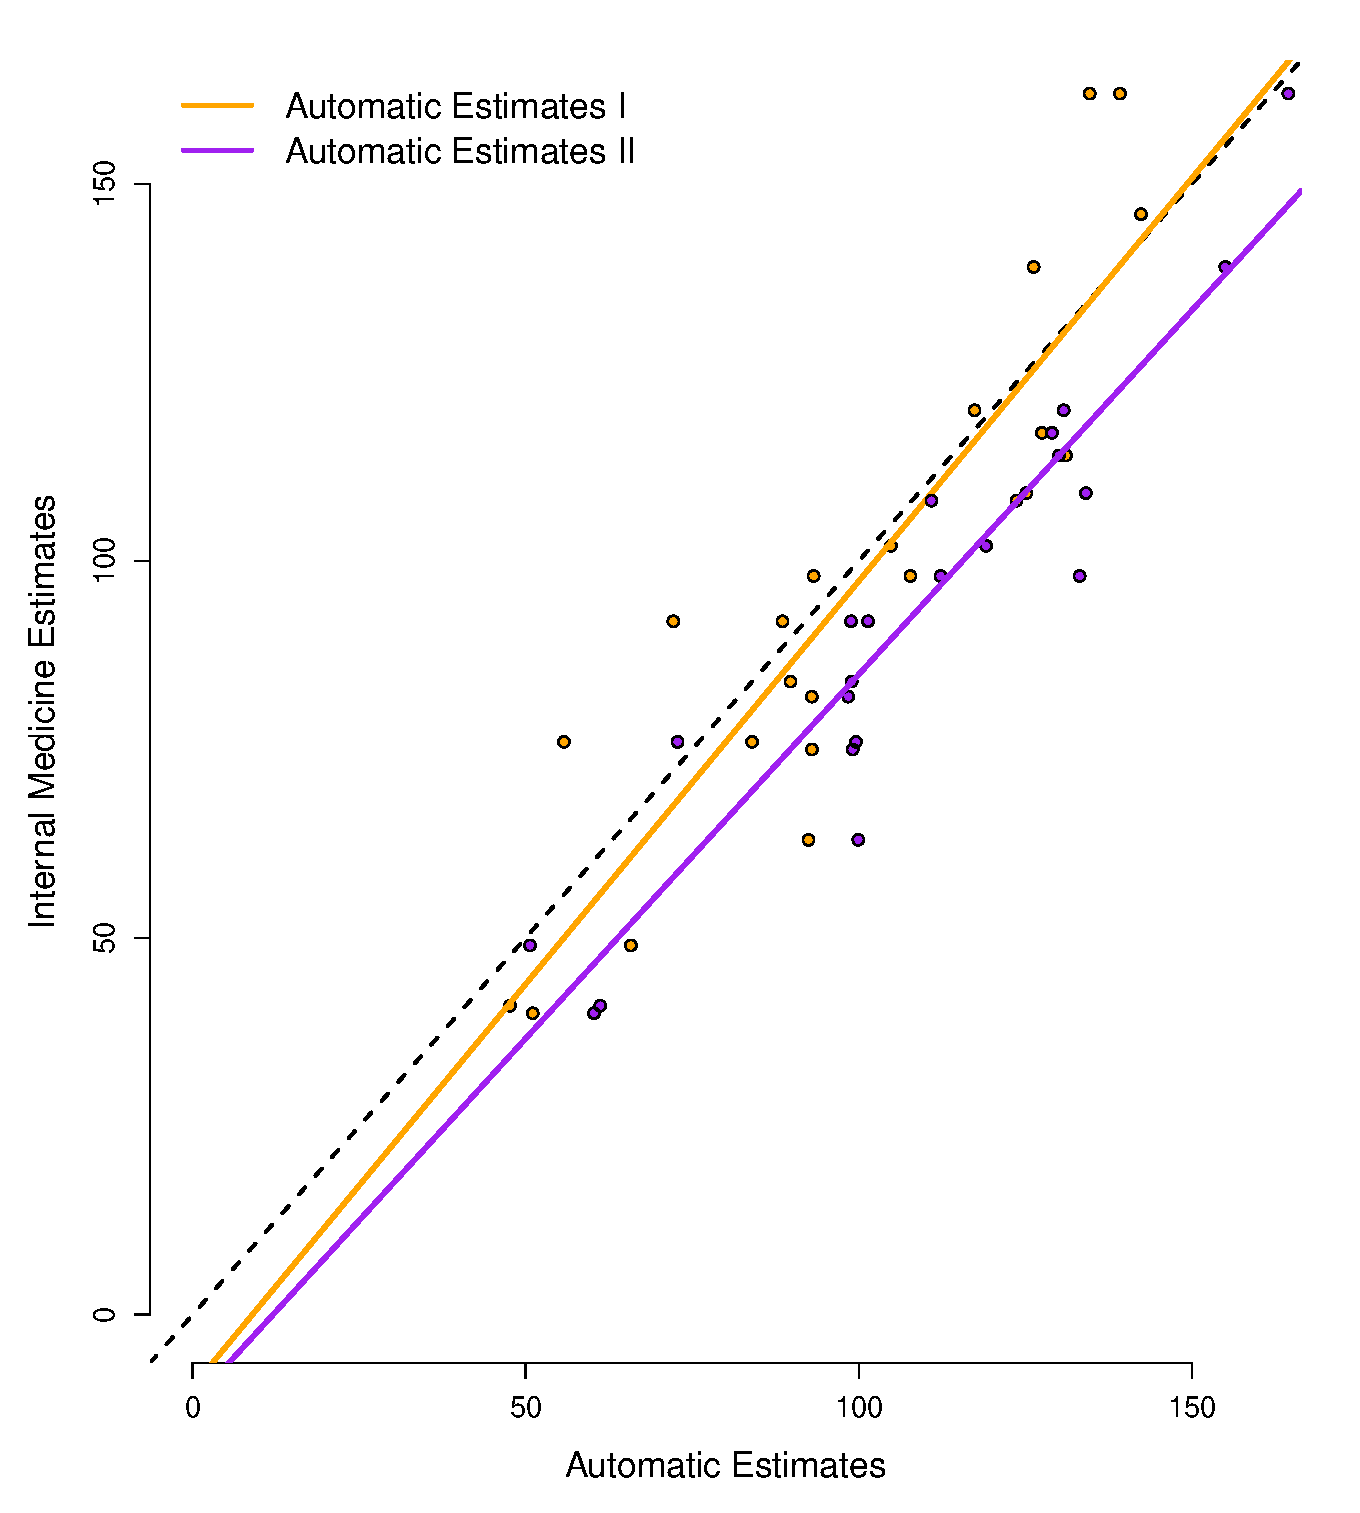
\includegraphics[width=0.6\linewidth]{linear-fit.pdf} 
%\caption{
%\label{fig:regression}
%Linear regression of automatic estimates from two different parameter settings
%against the estimates of a medical expert. The automatic estimates have an
%$\mathrm{R}^2$
%of 0.82 and 0.91, respectively and are statistically significant with a p-value
%on the order of machine precision ($2e^{-16}$).
%}
%\end{figure}

Table~\ref{tab:correlation} contains all pairwise correlations between all
participants of the study as well as two automatic estimates with different
parameter settings.
\begin{table}[!htbp] \centering 
\caption{Pairwise Pearson's correlation coefficients between novice (N1 - N10), expert ( E1 - E3 ) and
automatic (A1, A2) estimates.} 
\label{tab:correlation}
\resizebox{\textwidth}{!}{ 
\begin{tabular}{@{\extracolsep{5pt}} l|cccccccccc|ccc|cc} 
\\[-2.8ex] 
\hline
\hline 
\\[-1.8ex] 
   & N1 & N2 & N3 & N4 & N5 & N6 & N7 & N8 & N9 & N10 & E1 & E2 & E3 & A1 & A2 \\ 
\hline \\[-1.8ex] 
N1 & $1$ & $0.42$ & $0.34$ & $0.29$ & $0.33$ & $0.68$ & $0.32$ & $0.91$ & $0.56$ & $0.29$ & $0.52$ & $0.54$ & $0.36$ & $0.35$ & $0.52$ \\ 
N2 & $0.42$ & $1$ & $0.83$ & $0.93$ & $0.92$ & $0.85$ & $0.95$ & $0.56$ & $0.83$ & $0.93$ & $0.86$ & $0.91$ & $0.95$ & $0.91$ & $0.89$ \\ 
N3 & $0.34$ & $0.83$ & $1$ & $0.88$ & $0.92$ & $0.84$ & $0.90$ & $0.45$ & $0.70$ & $0.91$ & $0.80$ & $0.74$ & $0.88$ & $0.83$ & $0.83$ \\ 
N4 & $0.29$ & $0.93$ & $0.88$ & $1$ & $0.94$ & $0.80$ & $0.96$ & $0.42$ & $0.74$ & $0.97$ & $0.82$ & $0.83$ & $0.94$ & $0.92$ & $0.85$ \\ 
N5 & $0.33$ & $0.92$ & $0.92$ & $0.94$ & $1$ & $0.83$ & $0.93$ & $0.45$ & $0.72$ & $0.94$ & $0.83$ & $0.82$ & $0.91$ & $0.85$ & $0.85$ \\ 
N6 & $0.68$ & $0.85$ & $0.84$ & $0.80$ & $0.83$ & $1$ & $0.83$ & $0.75$ & $0.79$ & $0.82$ & $0.83$ & $0.84$ & $0.83$ & $0.83$ & $0.86$ \\ 
N7 & $0.32$ & $0.95$ & $0.90$ & $0.96$ & $0.93$ & $0.83$ & $1$ & $0.46$ & $0.83$ & $0.95$ & $0.80$ & $0.90$ & $0.97$ & $0.95$ & $0.89$ \\ 
N8 & $0.91$ & $0.56$ & $0.45$ & $0.42$ & $0.45$ & $0.75$ & $0.46$ & $1$ & $0.60$ & $0.45$ & $0.60$ & $0.66$ & $0.51$ & $0.51$ & $0.63$ \\ 
N9 & $0.56$ & $0.83$ & $0.70$ & $0.74$ & $0.72$ & $0.79$ & $0.83$ & $0.60$ & $1$ & $0.73$ & $0.82$ & $0.88$ & $0.82$ & $0.74$ & $0.78$ \\ 
N10 & $0.29$ & $0.93$ & $0.91$ & $0.97$ & $0.94$ & $0.82$ & $0.95$ & $0.45$ & $0.73$ & $1$ & $0.85$ & $0.80$ & $0.94$ & $0.91$ & $0.84$ \\ 
E1 & $0.52$ & $0.86$ & $0.80$ & $0.82$ & $0.83$ & $0.83$ & $0.80$ & $0.60$ & $0.82$ & $0.85$ & $1$ & $0.71$ & $0.82$ & $0.72$ & $0.77$ \\ 
E2 & $0.54$ & $0.91$ & $0.74$ & $0.83$ & $0.82$ & $0.84$ & $0.90$ & $0.66$ & $0.88$ & $0.80$ & $0.71$ & $1$ & $0.90$ & $0.88$ & $0.87$ \\ 
E3 & $0.36$ & $0.95$ & $0.88$ & $0.94$ & $0.91$ & $0.83$ & $0.97$ & $0.51$ & $0.82$ & $0.94$ & $0.82$ & $0.90$ & $1$ & $0.95$ & $0.90$ \\ 
A1 & $0.35$ & $0.91$ & $0.83$ & $0.92$ & $0.85$ & $0.83$ & $0.95$ & $0.51$ & $0.74$ & $0.91$ & $0.72$ & $0.88$ & $0.95$ & $1$ & $0.92$ \\ 
A2 & $0.52$ & $0.89$ & $0.83$ & $0.85$ & $0.85$ & $0.86$ & $0.89$ & $0.63$ & $0.78$ & $0.84$ & $0.77$ & $0.87$ & $0.90$ & $0.92$ & $1$ \\
\hline  
\end{tabular} 
}
\end{table} 

Table~\ref{tab:intercorrelation} shows the intra-and inter-correlation between
novice, expert and automatic estimates. The estimates from the novice N1 were
far off from any of the other novices and thus excluded from the results
reported here. The automatic estimates is more strongly correlated (0.85) to the
medical expert than the correlation within the group of medical experts
(0.81).The correlation among experts matches results of previous
studies~\cite{Ze2014,Jo2016}.  Thus, the precision of the proposed automatic
estimator is on par or even better than the medical experts.
\begin{table}[!htbp] 
\centering 
\caption{Inter- and intra-correlations (mean Pearson correlation coefficients)
among novice (excluding N1), expert and automated estimates.} 
\label{tab:intercorrelation} 
\begin{tabular}{@{\extracolsep{5pt}} l|ccc} 
\\[-2.8ex] 
\hline  
\hline 
\\[-1.8ex] 
   & Novice & Expert & Automatic \\ 
\hline \\[-1.8ex] 
Novice    & 0.78 & 0.83 & 0.82 \\
Expert    & 0.83 & 0.81 & 0.85 \\
Automatic & 0.82 & 0.85 & 0.92 \\
\hline 
\end{tabular} 
\end{table} 


\subsection{Gel Phantom Study}
\label{sec:groundtruth}
This evaluation is based on an eye phantom using 3D-printed “optic nerves”
(plastic discs) of known diameter embedded under gelatine orbs as described in
detail in~\cite{Ze2014}. The eye phantom produces ultrasound images that closely
resemble clinical ocular ultrasound images.
\begin{figure}
\centering
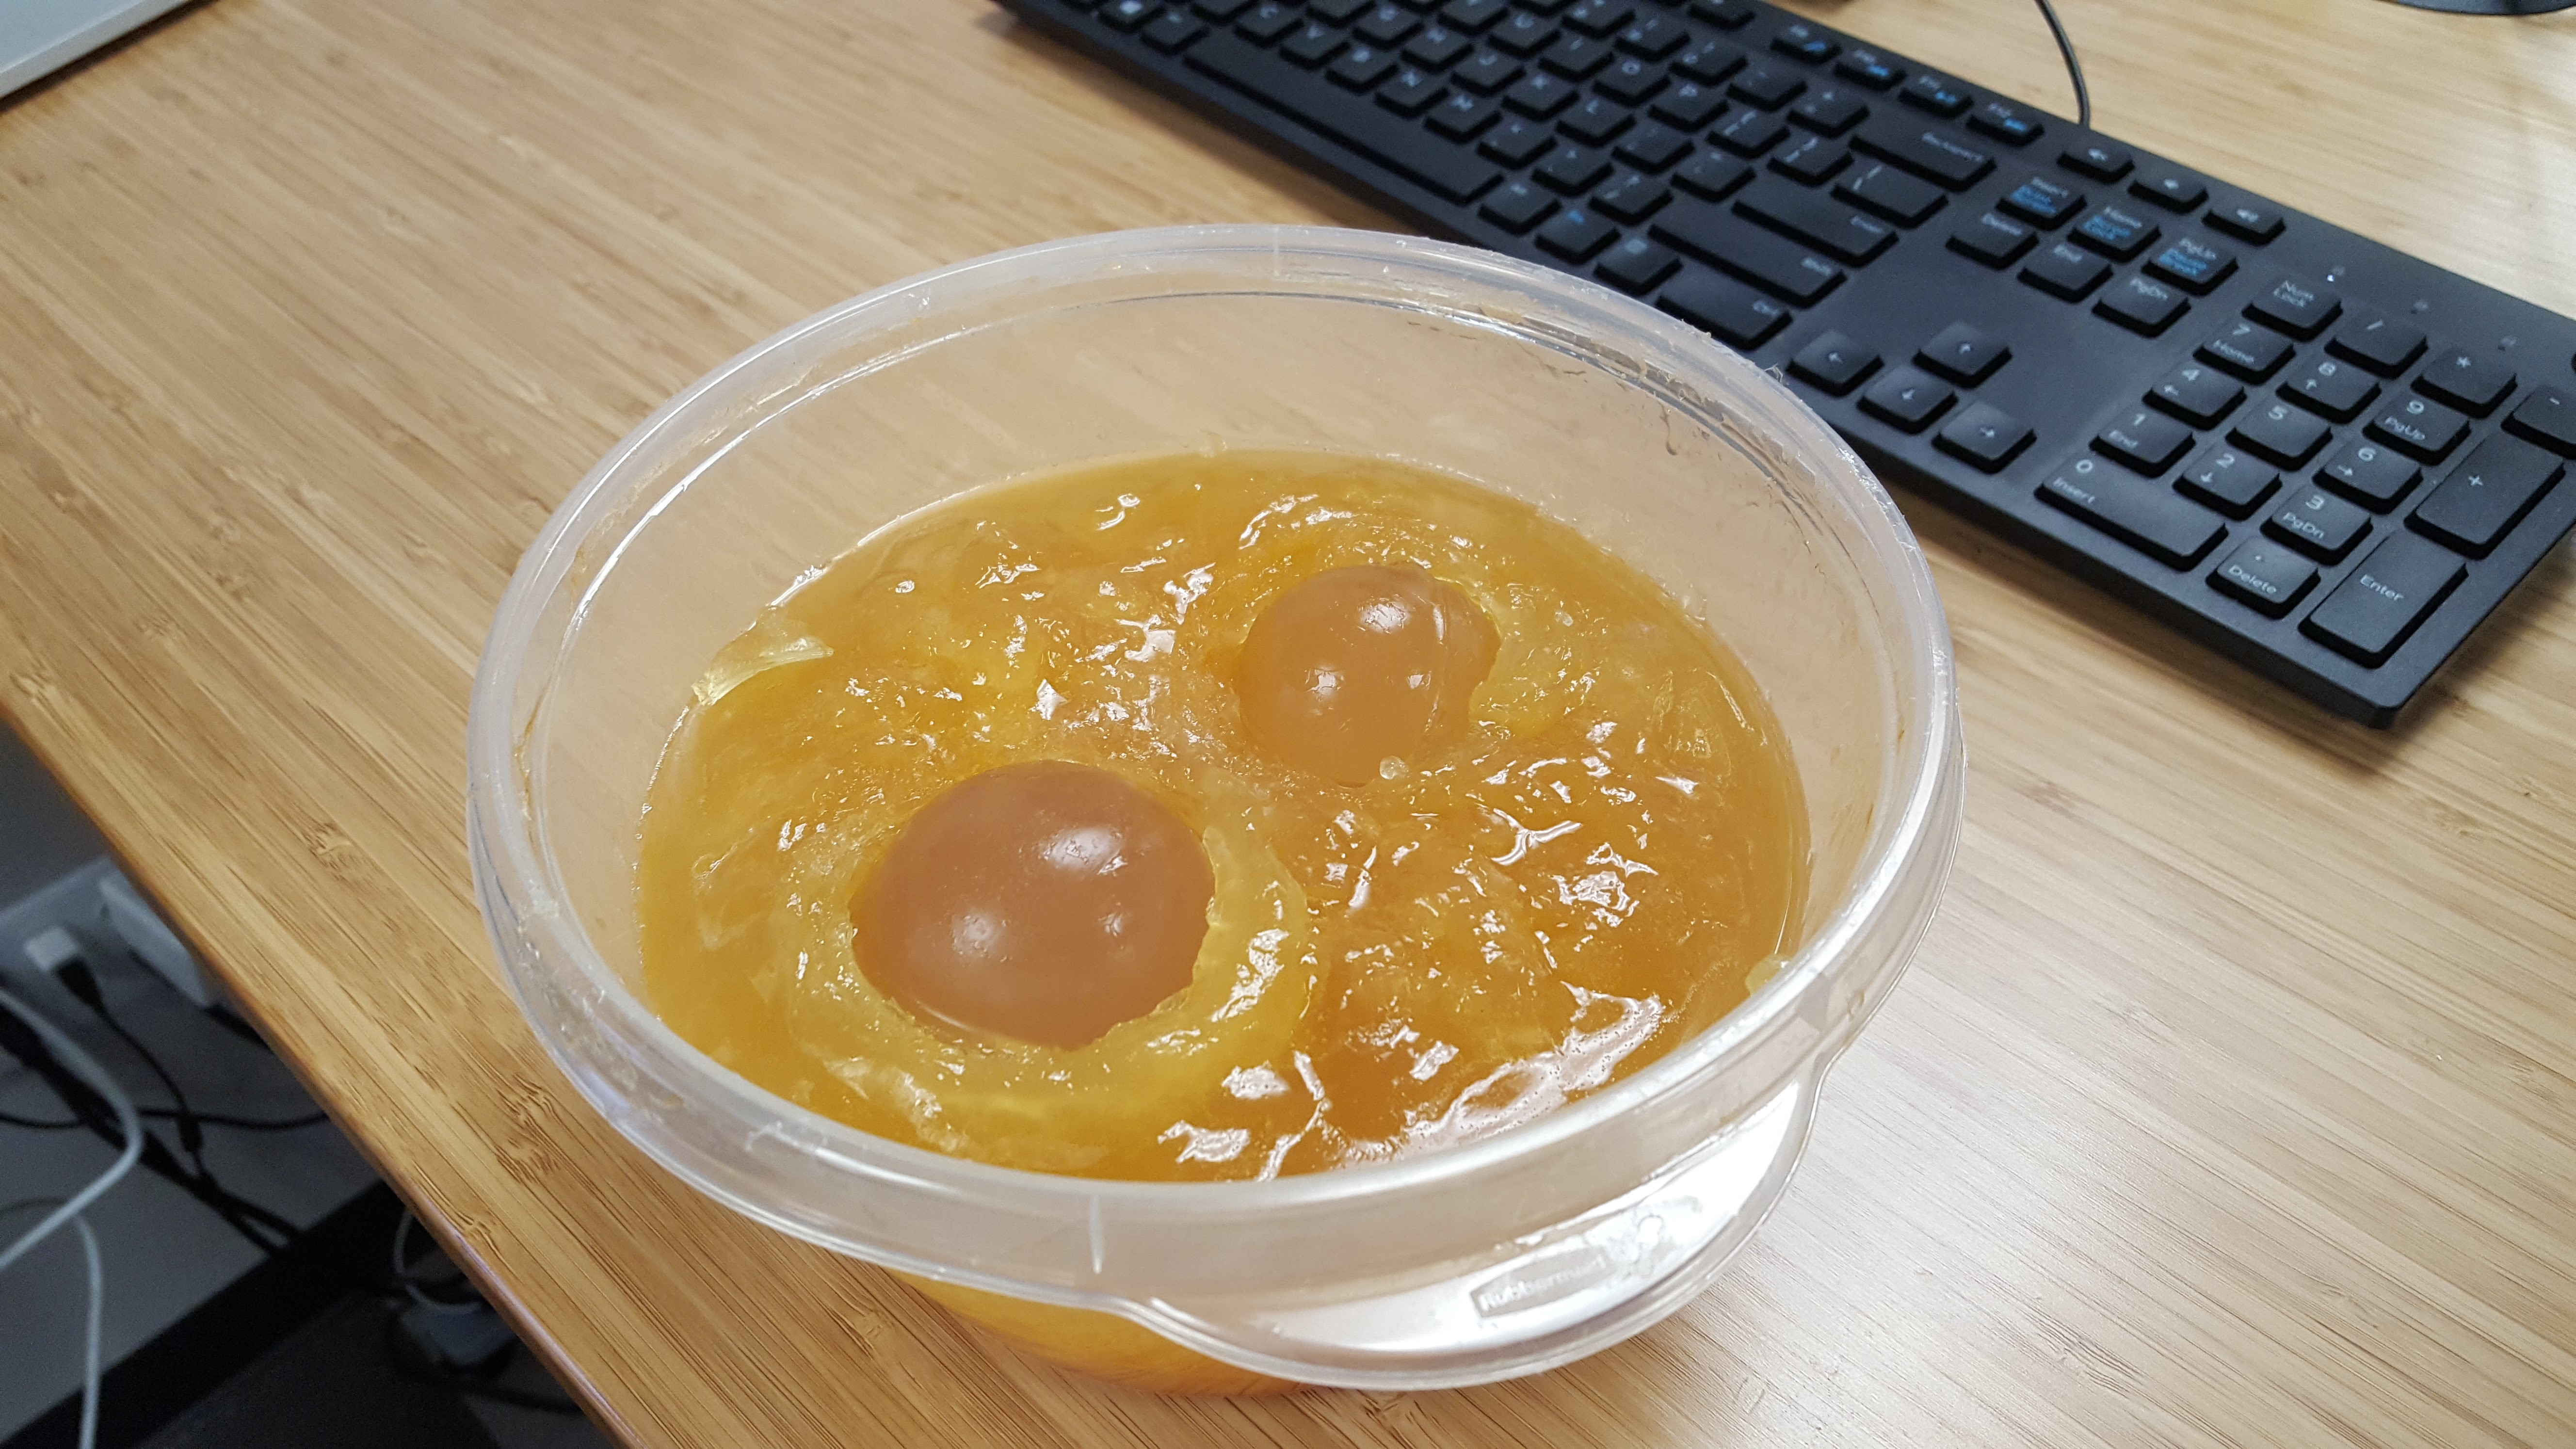
\includegraphics[width=0.7\linewidth]{phantom.jpg} 
\caption{
\label{fig:phantom}
Gelatine phantom for acquiring ultrasound images with know ground truth optic
nerve sheath diameters. The images from the phantom are a very realistic
approximation to images acquired through ocular ultrasound. 
}
\end{figure}

The goal of this evaluation is to check if an accurate estimate of the optic
nerve is possible with the proposed algorithm. We imaged the phantom using the
graphical user interface described in Section~\ref{sec:gui} connected to an
Interson linear array probe with 127 transducer elements and a pixel size of
0.8\,mm. A novice (non-medical imaging expert) used the graphical user-interface
,which shows B-mode images in real-time, to first locate the optic nerve. Once
the probe was positioned to deliver a good image of the optic nerve, as judged
by the novice user, the automatic estimation process was started and run
interactively for about 10 seconds. This resulted in approximately 40 to 50
optic nerve sheath diameter estimates. 

Table~\ref{tab:phantom} shows that, in this controlled setting, the means of the
automatic estimates are within less than +/- 5\,mm with a relatively tight
distribution of estimates around the ground truth diameter. A study on
intra-operator variations on the same type of phantom, but with higher
resolution ultrasound probes, reports an average bias of 0.33\,mm and standard
deviations of 0.64\,mm of the measurements~\cite{Jo2016}.  
\begin{table}
\centering
\caption{
Results of automatics diameter estimates on a gel eye phantom with known ground truth.
}
\label{tab:phantom}
\begin{tabular}{l|cc|ccc}
\\[-2.8ex] 
\hline  
\hline 
\\[-1.8ex]
Disc Size & Mean & Std. Deviation & Low.Quartile & Median & Up. Quartile \\
\hline
7mm & 7mm   & 1mm   & 6.4mm & 6.9mm & 7.7mm \\
6mm & 6.1mm & 1mm   & 5.8mm & 6.4mm & 6.6mm \\
5mm & 5.1mm & 1.4mm & 4.4mm & 4.9mm & 5.7mm \\
4mm & 4.4mm & 0.6mm & 4.2mm & 4.3mm & 4.5mm \\
3mm & 3.4mm & 1.1mm & 2.9mm & 3.2mm & 3.5mm \\
\hline 
\end{tabular}
\end{table}

\section{Conclusion}
The results presented indicate that the algorithm performs well in a controlled
setting.  A retrospective analysis of clinical images indicate that our system
performs similar to an expert, and a phantom study using 3D printed optic
nerves of known diameter suggests that our system is accurate.

The next step is to integrate an image quality estimation algorithm, so that
high quality images of the optic nerve can be automatically identified as a
probe is swept over the eye. This will eliminate the need for the operator to
view, interpret, or make measurements on an ultrasound image when using it to
assess a dilated optic nerve sheath, as indicative of increased intracranial
pressure. Ultimately, we aim for a system that can be used by novice operators
with minimal ultrasound experience. The system will report when a sufficient
image has been acquired, and it will automatically determine if the diameter of
the optic nerve is greater than 5mm, thereby indicating increased intracranial
pressure associated with mild or more severe TBI~\cite{Ma2015}.

The long term goal is to develop a lightweight portable ultrasound
system that, in addition to automated diagnosis of TBI, includes automatic
diagnosis tools for pneumothorax (detached lung) and internal bleeding.

%
% ---- Bibliography ----
%
\begin{thebibliography}{}
%
\bibitem[Du2011]{Du2011}
Dubourg, Julie, et al. 
Ultrasonography of optic nerve sheath diameter for detection of raised
intracranial pressure: a systematic review and meta-analysis.
Intensive care medicine 37.7 (2011): 1059-1068.

%\bibitem[Du2012]{Du2012}
%Dubost, Clément, et al. 
%Optic Nerve Sheath Diameter Used as Ultrasonographic Assessment of the Incidence
%of Raised Intracranial Pressure in PreeclampsiaA Pilot Study.  
%The Journal of the American Society of Anesthesiologists 116.5 (2012): 1066-1071.

%\bibitem[Ga2005]{Ga2005}
%Garcia, Julian PS, et al. 
%Optic nerve measurements by 3D ultrasound-based coronal" C-scan" imaging.
%Ophthalmic Surgery, Lasers and Imaging Retina 36.2 (2005): 142-146.

\bibitem[Jo2016]{Jo2016}
Johnson, Garrett GRJ, et al. 
Estimating the accuracy of optic nerve sheath diameter measurement using a
pocket-sized, handheld ultrasound on a simulation model.  Critical Ultrasound
Journal 8.1 (2016): 18.

\bibitem[Ki2008]{Ki2008}
Kimberly, Heidi Harbison, et al. 
Correlation of optic nerve sheath diameter with direct measurement of
intracranial pressure.
Academic Emergency Medicine 15.2 (2008): 201-204.

\bibitem[Ma2015]{Ma2015}
Maissan IM , Dirven PJ , Haitsma IK , Hoeks SE , Gommers D , Stolker RJ 
Ultrasonographic measured optic nerve sheath diameter as an accurate and quick
monitor for changes in intracranial pressure. 
J Neurosurg. 2015 Sep;123(3):7437

\bibitem[Mo2009]{Mo2009}
Moretti, Riccardo, et al. 
Reliability of optic nerve ultrasound for the evaluation of patients with
spontaneous intracranial hemorrhage.
Neurocritical care 11.3 (2009): 406.

\bibitem[Ra2011]{Ra2011}
Rajajee, Venkatakrishna, et al. 
Optic nerve ultrasound for the detection of raised intracranial pressure. 
Neurocritical care 15.3 (2011): 506-515.

\bibitem[Ro2011]{Ro2011}
Rosenberg, Jamie B., et al. 
Non-invasive methods of estimating intracranial pressure.
Neurocritical care 15.3 (2011): 599-608.

\bibitem[Se1981]{Se1981}
Seelig, John M., et al. 
Traumatic acute subdural hematoma: major mortality reduction in comatose
patients treated within four hours.
New England Journal of Medicine 304.25 (1981): 1511-1518.

\bibitem[Ze2014]{Ze2014}
Zeiler, F. A., et al. 
A unique model for ONSD Part II: inter/intra-operator variability. 
Can J Neurol Sci 41 (2014): 430-435.



\end{thebibliography}

\end{document}
